\chapter{Agent harness architecture}

\section{Engineering principles}

The model produces predictions; the agent couples them to a task and tool loop; the harness owns execution mechanics; a framework is reusable software for assembling applications. Codex and Claude Code already provide substantial runtime functionality. The external extension should coordinate task contracts, identity, workspace isolation, policies, independent verification, approval and durable records without replicating token management or tool dispatch. Native and external layers are complementary rather than competing.\src{O6,O7,A9}

\section{Implementation approach}

Place the policy and verification stages outside the agent workspace. Route requests through a provider adapter with a narrow interface: execute a task in an allocated directory, return exit status and evidence. An immutable configuration image and a task-scoped credential broker define the outer boundary. Record provider version, policy version and base commit. Keep acceptance tests in a trusted checkout or independent runner.

\section{Verification and limitations}

A native permission prompt is not organizational approval to merge. The orchestrator must fail closed when an adapter is unsupported, the policy cannot be loaded or verification cannot be completed.

Figure~\ref{fig:d2} illustrates the conceptual flow from External task control to Trusted verification. The edges describe the proposed integration or control relationship, not undocumented internal calls.

\begin{figure}[htbp]\centering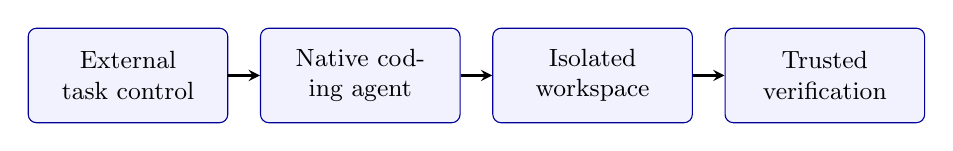
\begin{tikzpicture}[nodebox/.style={draw=blue!60!black,fill=blue!5,rounded corners=3pt,minimum height=12mm,text width=23mm,align=center,font=\small},>=stealth]
\node[nodebox] (n0) at (0.00,0.00) {External task control};
\node[nodebox] (n1) at (2.95,0.00) {Native coding agent};
\node[nodebox] (n2) at (5.90,0.00) {Isolated workspace};
\node[nodebox] (n3) at (8.85,0.00) {Trusted verification};
\draw[->,thick] (n0.east) -- (n1.west);
\draw[->,thick] (n1.east) -- (n2.west);
\draw[->,thick] (n2.east) -- (n3.west);
\end{tikzpicture}
\caption{Native and external harness responsibilities (conceptual view).}\label{fig:d2}\end{figure}

\section{Chapter conclusion}

Apply the stated verification criteria before expanding the scope of this workflow. Record deviations, evidence and unresolved risks in the task record.
